%
% firmware.tex
%
% Copyright (C) 2022 by SpaceLab.
%
% OBDH 2.0 Module
%
% This work is licensed under the Creative Commons Attribution-ShareAlike 4.0
% International License. To view a copy of this license,
% visit http://creativecommons.org/licenses/by-sa/4.0/.
%

%
% \brief Firmware project slides.
%
% \author Gabriel Mariano Marcelino <gabriel.mm8@gmail.com>
% \author Bruno Benedetti <brunobenedetti45@gmail.com>
%
% \version 0.1.0
%
% \date 2022/07/28
%


\begin{frame}{Overview}

    \begin{columns}[t]
        \begin{column}[t]{0.6\textwidth}
            \begin{itemize}
                \item Language: C
                \vspace{0.3cm}
                \item OS: FreeRTOS v10.2.1
                \vspace{0.3cm}
                \item Customized for a given mission
            \end{itemize}
        \end{column}
        \begin{column}[t]{0.4\textwidth}
            \begin{figure}[!ht]
                \begin{center}
                    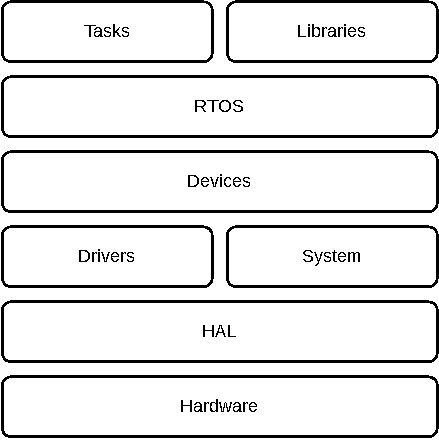
\includegraphics[width=4cm]{figures/obdh2-layers.pdf}
                \end{center}
            \end{figure}
        \end{column}
    \end{columns}

\end{frame}

% #########################################################################
% #########################################################################

\begin{frame}{System Tasks}

\begin{table}[!h]\tiny
    \centering
    \label{tab:firmware-tasks}
    \begin{tabular}{lccccc}
        \toprule[1.5pt]
        \textbf{Name}          & \textbf{Priority} & \textbf{Initial delay [ms]} & \textbf{Period [ms]} & \textbf{Stack [bytes]} \\
        \midrule
        Antenna deployment     & Highest & 0      & Aperiodic & 150  \\
        Antenna reading        & Medium  & 2000   & 60000     & 150  \\
        Beacon                 & High    & 1000   & 60000     & 1000 \\
        Data log               & Medium  & 2000   & 600000    & 225  \\
        EDC reading            & Medium  & 2000   & 60000     & 300  \\
        EPS reading            & Medium  & 2000   & 60000     & 384  \\
        Heartbeat              & Lowest  & 2000   & 500       & 160  \\
        Housekeeping           & Medium  & 2000   & 10000     & 160  \\
        Read sensors           & Medium  & 2000   & 60000     & 140  \\
        Startup (boot)         & Highest & 0      & Aperiodic & 350  \\
        System reset           & Medium    & 0    & 36000000  & 128  \\
        Telecommand processing & High    & 10000   & 5000      & 500  \\
        Time control           & Medium  & 1000   & 1000      & 128  \\
        TTC reading            & Medium  & 2000   & 60000     & 384  \\
        Watchdog reset         & Lowest  & 0      & 100       & 150  \\
        \bottomrule[1.5pt]
    \end{tabular}
\end{table}

\end{frame}

\begin{frame}{System Tasks}

    \begin{itemize}
        \item \textbf{Antenna deployment}: This task deploys the antenna module just after the satellite ejection.
        \item \textbf{Peripherals data reading}: Each peripheral has a unique task for data reading.
        \item \textbf{Beacon}: The Beacon task transmits a data package that contais basic telemetry data of the satellite at every 60 seconds.
        \item \textbf{Data log}: This tasks saves the housekeeping data of the satellite in the flash memory at every 10 minutes.
        \item \textbf{Heartbeat}: The Heartbeat task keeps blinking an status LED at a rate of 1 Hz.
        \item \textbf{Housekeeping}: This task manages the general operation of the OBDH.
    \end{itemize}

\end{frame}

\begin{frame}{System Tasks}

    \begin{itemize}
        \item \textbf{Read sensors}: This task reads the internal sensors of the OBDH at every 60 seconds.
        \item \textbf{Startup (boot)}: All devices, libraries and data structures are initialized in this task.
        \item \textbf{System reset}: This task resets the microcontroller by software at every 10 hours.
        \item \textbf{Telecommand processing}: This task processes all incoming telecomands. 
        \item \textbf{Time control}: This task is responsible for the time management of the system.
        \item \textbf{Watchdog reset}: This task resets the internal and external watchdog timer at every 100 ms.
    \end{itemize}

\end{frame}

% #########################################################################
% #########################################################################

\begin{frame}{System Parameters}

\begin{table}[!htb]\tiny
    \centering
    \label{tab:vars-and-pars}
    \begin{tabular}{cll}
        \toprule[1.5pt]
        \textbf{ID} & \textbf{Name/Description} & \textbf{Type}\\
        \midrule
        0   & Time counter in milliseconds                            & uint32 \\
        1   & Temperature of the $\mu$C in Kelvin                     & uint16 \\
        2   & Input current in mA                                     & uint16 \\
        3   & Input voltage in mV                                     & uint16 \\
        4   & Last reset cause                                        & uint8 \\
        5   & Reset counter                                           & uint16 \\
        6   & Last valid telecommand (uplink packet ID)               & uint8  \\
        7   & Temperature of the radio in Kelvin                      & uint16 \\
        8   & RSSI of the last valid telecommand                      & uint16 \\
        9   & Temperature of the antenna in Kelvin                    & uint16 \\
        10  & Antenna status bits                                     & uint16 \\
        11  & Hardware version                                        & uint8 \\
        12  & Firmware version (ex.: ``v1.2.3'' = 0x00010203)         & uint32 \\
        13  & Mode (``Normal'' = 0, ``Hibernation'' = 1)              & uint8 \\
        14  & Timestamp of the last mode change                       & uint32 \\
        15  & Mode duration in sec. (valid only in hibernation mode)  & uint32 \\
        16  & Initial hibernation executed                            & boolean \\
        17  & Initial hibernation time counter (minutes)              & uint8 \\
        18  & Antenna deployment executed                             & boolean \\
        19  & Antenna deployment counter                              & uint8 \\
        \bottomrule[1.5pt]
    \end{tabular}
\end{table}

\end{frame}

% #########################################################################
% #########################################################################

\begin{frame}{Firmware: Development Environment}

    \begin{columns}[t]
        \begin{column}[t]{0.6\textwidth}
            \begin{itemize}
                \item Hardware: Engineering Model (EM)
                \vspace{0.4cm}
                \item Programmer: Texas Instruments MSP-FET programmer
                \vspace{0.4cm}
                \item IDE/Compiler: Code Composer Studio
                \vspace{0.4cm}
            \end{itemize}
        \end{column}
        \begin{column}[t]{0.4\textwidth}
            \begin{figure}[!ht]
                \begin{center}
                    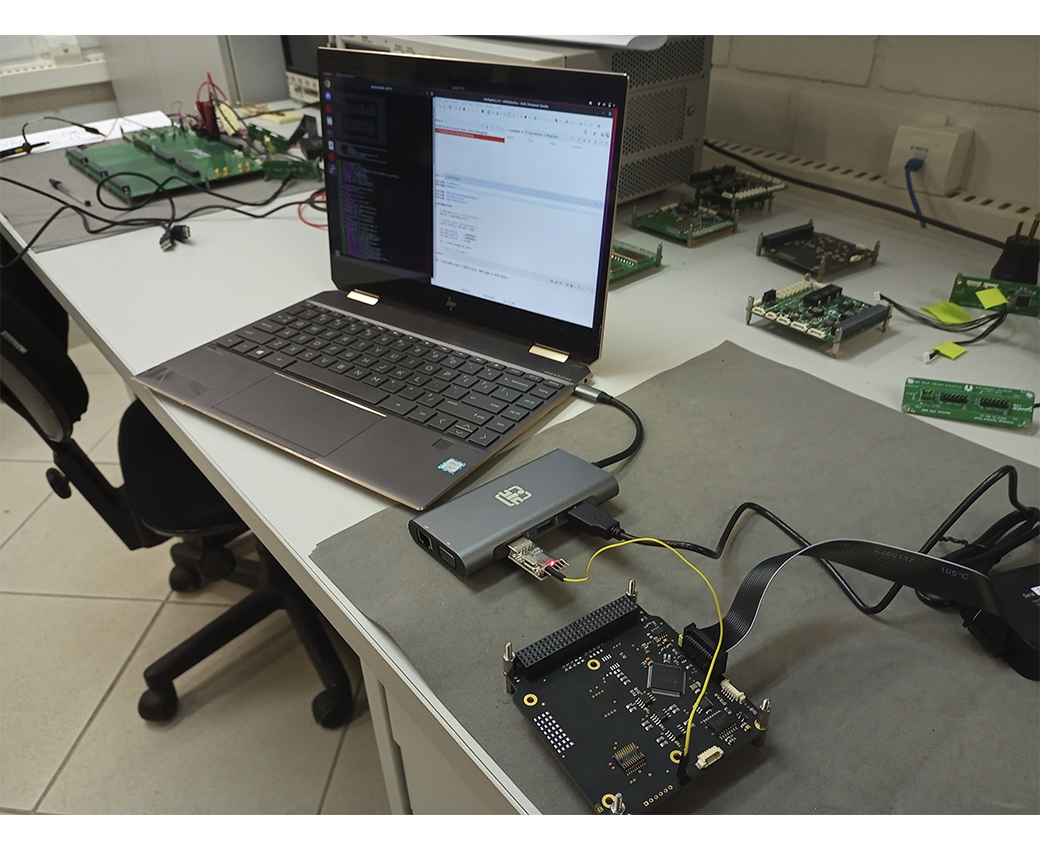
\includegraphics[width=4cm]{figures/obdh2-bench.png}
                \end{center}
            \end{figure}
        \end{column}
    \end{columns}

\end{frame}

% #########################################################################
% #########################################################################

\begin{frame}{Verification \& Validation}

    \begin{itemize}
        \item Unit tests framework: \href{https://cmocka.org/}{\textcolor{blue}{\underline{CMocka}}}
        \vspace{0.5cm}
        \item Static analysis tool: \href{https://cppcheck.sourceforge.io/}{\textcolor{blue}{\underline{CppCheck}}}
        \vspace{0.5cm}
        \item Code style standard: \href{https://www.misra.org.uk/}{\textcolor{blue}{\underline{MISRA-C 2012}}}
    \end{itemize}

\end{frame}

\begin{frame}{Verification \& Validation: TDD Flow}

    \begin{figure}[!ht]
        \begin{center}
            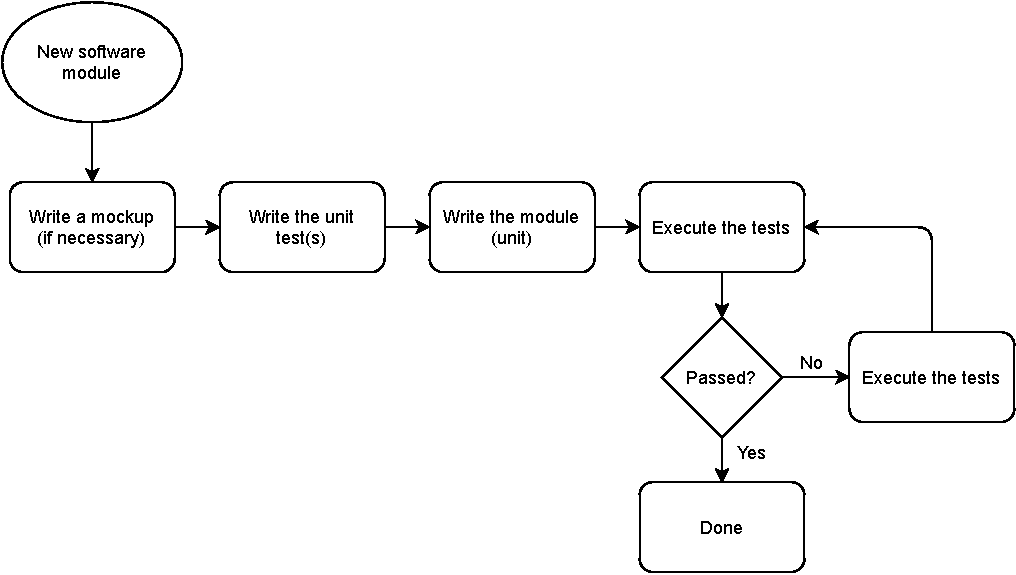
\includegraphics[width=11cm]{figures/tdd-flow.pdf}
        \end{center}
    \end{figure}

\end{frame}

\begin{frame}{Verification \& Validation: Development Flow}

    \begin{figure}[!ht]
        \begin{center}
            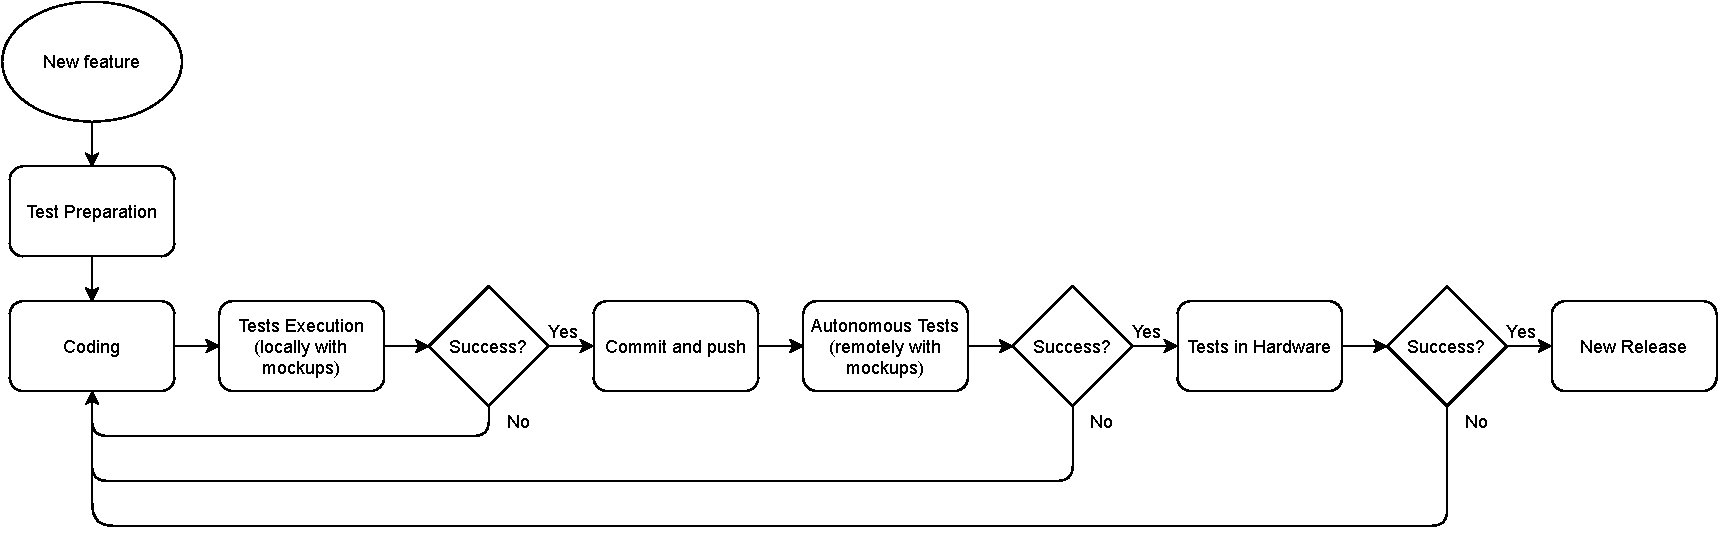
\includegraphics[width=11cm]{figures/dev-flow.pdf}
        \end{center}
    \end{figure}

\end{frame}